\documentclass{article}

% if you need to pass options to natbib, use, e.g.:
%     \PassOptionsToPackage{numbers, compress}{natbib}
% before loading neurips_2021

% ready for submission
%\PassOptionsToPackage{numbers}{natbib}
\usepackage[preprint]{neurips_2021}

% to compile a preprint version, e.g., for submission to arXiv, add add the
% [preprint] option:
%     \usepackage[preprint]{neurips_2021}

% to compile a camera-ready version, add the [final] option, e.g.:
%     \usepackage[final]{neurips_2021}

% to avoid loading the natbib package, add option nonatbib:
%    \usepackage[nonatbib]{neurips_2021}
\usepackage{subfig}

\usepackage[utf8]{inputenc} % allow utf-8 input
\usepackage[T1]{fontenc}    % use 8-bit T1 fonts
\usepackage[colorlinks=true, linkcolor=blue, citecolor=blue,urlcolor=black]{hyperref}  
\usepackage{url}            % simple URL typesetting
\usepackage{booktabs}       % professional-quality tables
\usepackage{amsfonts}       % blackboard math symbols
\usepackage{nicefrac}       % compact symbols for 1/2, etc.
\usepackage{microtype}      % microtypography
\usepackage{xcolor}         % colors

\definecolor{Green}{rgb}{0.13, 0.65, 0.3}
\definecolor{Amber}{rgb}{0.3, 0.5, 1.0}
\usepackage[]{color-edits}
\addauthor{TJ}{red}


%!TEX root=main.tex
%\PassOptionsToPackage{numbers}{natbib}
%\usepackage{neurips_2021}
\usepackage[utf8]{inputenc} % allow utf-8 input
\usepackage[T1]{fontenc}    % use 8-bit T1 fonts

\usepackage{amsthm}
\usepackage[algo2e, ruled, vlined]{algorithm2e}
\usepackage{algorithmicx}
\usepackage{algorithm}
\usepackage[noend]{algcompatible}
\usepackage{bbm}      
\usepackage{mathtools}    
\usepackage{amsopn}
\usepackage{amssymb}
\usepackage{graphicx}
\usepackage{xcolor}
%\usepackage{footnotehyper}

\definecolor{Green}{rgb}{0.13, 0.65, 0.3}
\definecolor{Amber}{rgb}{0.3, 0.5, 1.0}
\usepackage[]{color-edits}
\addauthor{HL}{Green}
\addauthor{TJ}{Amber}
\usepackage{comment}

\usepackage[skins,theorems]{tcolorbox} 
\tcbset{highlight math style={enhanced,colframe=red,colback=white,arc=0pt,boxrule=1pt}} 
%!TEX root=main.tex
\newcommand{\theset}[2]{ \left\{ {#1} \,:\, {#2} \right\} }
\newcommand{\inner}[1]{ \left\langle {#1} \right\rangle }
\newcommand{\Ind}[1]{ \field{I}{\left\{{#1}\right\}} }
\newcommand{\ind}{\field{I}}
\newcommand{\Indt}[1]{ \field{I}_t{\left({#1}\right)} }
\newcommand{\Indtau}[1]{ \field{I}_\tau{\left({#1}\right)} }
\newcommand{\eye}[1]{ \boldsymbol{I}_{#1} }
\newcommand{\norm}[1]{\left\|{#1}\right\|}
%\newcommand{\trace}[1]{\text{tr}\left({#1}\right)}
\newcommand{\trace}[1]{\textsc{tr}({#1})}
\newcommand{\diag}[1]{\mathrm{diag}\!\left\{{#1}\right\}}

\newcommand{\defeq}{\stackrel{\rm def}{=}}
\newcommand{\sgn}{\mbox{\sc sgn}}
\newcommand{\scI}{\mathcal{I}}
\newcommand{\scO}{\mathcal{O}}
\newcommand{\scN}{\mathcal{N}}

\newcommand{\dt}{\displaystyle}
\renewcommand{\ss}{\subseteq}
\newcommand{\wh}[1]{\widehat{#1}}
\newcommand{\ve}{\varepsilon}
\newcommand{\hlambda}{\wh{\lambda}}
\newcommand{\yhat}{\wh{y}}
\newcommand{\wb}{\overline}

%\newcommand{\gap}{\ensuremath{\mathtt{gap}}}
\newcommand{\gap}{\Delta}
\newcommand{\hatl}{\widehat{\ell}}
\newcommand{\hatL}{\widehat{L}}
\newcommand{\hatq}{\hat{q}}
\newcommand{\hatp}{\hat{p}}
\newcommand{\whatp}{\widehat{p}}
\newcommand{\whatq}{\widehat{q}}

\newcommand{\whatQ}{\widehat{Q}}
\newcommand{\whatV}{\widehat{V}}

\newcommand{\wtilQ}{\widetilde{Q}}
\newcommand{\wtilV}{\widetilde{V}}

\newcommand{\tilq}{\tilde{q}}
\newcommand{\tilp}{\tilde{p}}
\newcommand{\clip}{\text{clip}}
\newcommand{\wtilq}{\widetilde{q}}
\newcommand{\wtilp}{\widetilde{p}}
\newcommand{\wtill}{\widetilde{\ell}}
\newcommand{\selfterm}{\mathbb{G}}

\newcommand{\hDelta}{\wh{\Delta}}
\newcommand{\hdelta}{\wh{\delta}}
\newcommand{\spin}{\{-1,+1\}}
\newcommand{\pbar}{\overline{p}}

%%%%%%%%%%%%%%%%%%%%%%%%


\theoremstyle{theorem} 
	\newtheorem{theorem}{Theorem}[subsection]
	\newtheorem{lemma}[theorem]{Lemma}
	\newtheorem{observation}[theorem]{Observation}
	\newtheorem{corollary}[theorem]{Corollary}
	\newtheorem{proposition}[theorem]{Proposition}
	\newtheorem{definition}[theorem]{Definition}
	\newtheorem{remark}[theorem]{Remark}
	\newtheorem{assumption}{Assumption}

% magic code for numberings 
\renewcommand{\thetheorem}{%
	\ifnum\value{subsection}>0 
	\thesubsection
	\else
	\thesection
	\fi
	.\arabic{theorem}%
}


\DeclareMathOperator{\val}{val}
\DeclareMathOperator{\spa}{sp}
\DeclareMathOperator{\solve}{solve}
\allowdisplaybreaks

% Packages hyperref and algorithmic misbehave sometimes.  We can fix
% this with the following command.
%\newcommand{\theHalgorithm}{\arabic{algorithm}}

\usepackage{amsmath}
\DeclareMathOperator*{\argmin}{\arg\!\min}
\DeclareMathOperator*{\argmax}{\arg\!\max}

\newcommand{\agmin}[1]{\underset{#1}{\argmin\,} }
\newcommand{\agmax}[1]{\underset{#1}{\argmax\,} }
\newcommand{\dotprod}[2]{\langle{#1},{#2}\rangle}
\usepackage{amsthm}
\usepackage{amsmath}
\usepackage{amssymb}
\usepackage{graphicx}
\usepackage{mathtools}
\usepackage{enumerate}
\usepackage{enumitem}
\usepackage{footnote}
\usepackage{float}
\usepackage{xspace}
\usepackage{multirow}
\usepackage{nicefrac}
\usepackage{wrapfig}
\usepackage{framed}
\usepackage{url}
\usepackage{tikz}
\usetikzlibrary{arrows,chains,matrix,positioning,scopes}

\newcommand{\push}{\hspace{0pt plus 1 filll} }	

\newcommand{\calA}{{\mathcal{A}}}
\newcommand{\calB}{{\mathcal{B}}}
\newcommand{\calC}{{\mathcal{C}}}
\newcommand{\calH}{{\mathcal{H}}}
\newcommand{\calL}{{\mathcal{L}}}
\newcommand{\calU}{{\mathcal{U}}}
\newcommand{\calX}{{\mathcal{X}}}
\newcommand{\calY}{{\mathcal{Y}}}
\newcommand{\calS}{{\mathcal{S}}}
\newcommand{\calI}{{\mathcal{I}}}
\newcommand{\calD}{{\mathcal{D}}}
\newcommand{\calK}{{\mathcal{K}}}
\newcommand{\calE}{{\mathcal{E}}}
\newcommand{\calR}{{\mathcal{R}}}
\newcommand{\calT}{{\mathcal{T}}}
\newcommand{\calP}{{\mathcal{P}}}
\newcommand{\calZ}{{\mathcal{Z}}}
\newcommand{\calM}{{\mathcal{M}}}
\newcommand{\calN}{{\mathcal{N}}}
\newcommand{\calF}{{\mathcal{F}}}
\newcommand{\calV}{{\mathcal{V}}}
\newcommand{\calQ}{{\mathcal{Q}}}
\newcommand{\ips}{\wh{r}}
\newcommand{\whpi}{\wh{\pi}}
\newcommand{\whE}{\wh{\E}}
\newcommand{\whV}{\wh{V}}
\newcommand{\reg}{{\mathcal{R}}}
\newcommand{\breg}{{\mathcal{\bar{R}}}}
\newcommand{\hmu}{\wh{\mu}}
\newcommand{\tmu}{\wt{\mu}}
\newcommand{\one}{\boldsymbol{1}}
\newcommand{\loss}{\ell}
\newcommand{\hloss}{\wh{\ell}}
\newcommand{\bloss}{\bar{\ell}}
\newcommand{\tloss}{\wt{\ell}}
\newcommand{\htheta}{\wh{\theta}}

% special commands 
\newcommand{\paralog}{\beta}
\newcommand{\cnt}{B}
\newcommand{\cons}{J}
\newcommand{\pcons}{\iota}
\newcommand{\gapmin}{\Delta_{\textsc{min}}}
\newcommand{\dmax}{d_{\textsc{max}}}
\DeclareMathOperator{\polylog}{{\ensuremath{\mathrm{polylog}}}}

\newcommand{\bz}{\boldsymbol{z}}
\newcommand{\bx}{\boldsymbol{x}}
\newcommand{\br}{\boldsymbol{r}}
\newcommand{\bX}{\boldsymbol{X}}
\newcommand{\bu}{\boldsymbol{u}}
\newcommand{\by}{\boldsymbol{y}}
\newcommand{\bY}{\boldsymbol{Y}}
\newcommand{\bg}{\boldsymbol{g}}
\newcommand{\ba}{\boldsymbol{a}}
\newcommand{\be}{\boldsymbol{e}}
\newcommand{\bq}{\boldsymbol{q}}
\newcommand{\bp}{\boldsymbol{p}}
\newcommand{\bZ}{\boldsymbol{Z}}
\newcommand{\bS}{\boldsymbol{S}}
\newcommand{\bw}{\boldsymbol{w}}
\newcommand{\bW}{\boldsymbol{W}}
\newcommand{\bU}{\boldsymbol{U}}
\newcommand{\bv}{\boldsymbol{v}}
\newcommand{\bzero}{\boldsymbol{0}}

\newcommand{\blue}[1]{{\color{blue}#1}}

\DeclareMathOperator*{\range}{range}
\DeclareMathOperator*{\mydet}{det_{+}}

\newcommand{\field}[1]{\mathbb{#1}}
\newcommand{\fY}{\field{Y}}
\newcommand{\fX}{\field{X}}
\newcommand{\fH}{\field{H}}
\newcommand{\fR}{\field{R}}
\newcommand{\fB}{\field{B}}
\newcommand{\fS}{\field{S}}
\newcommand{\fN}{\field{N}}
\newcommand{\E}{\field{E}}
\newcommand{\var}{\field{V}}
\renewcommand{\P}{\field{P}}
%\newcommand{\inner}[1]{ \left\langle {#1} \right\rangle }
\newcommand{\RE}{{\text{\rm RE}}}
\newcommand{\KL}{{\text{\rm KL}}}
\newcommand{\LCB}{{\text{\rm LCB}}}
\newcommand{\Reg}{{\text{\rm Reg}}}
\newcommand{\EReg}{{\text{\rm EstReg}}}
\newcommand{\Rel}{{\text{\rm Rel}}}
%\newcommand{\ERM}{{\text{\rm ERM}}\xspace}

\renewcommand{\ss}{\subseteq}
\newcommand{\wt}{\widetilde}
\newcommand{\pred}{\yhat}
\newcommand{\bigand}{\bigwedge\limits}

\newcommand{\normt}[1]{\norm{#1}_{t}}
\newcommand{\dualnormt}[1]{\norm{#1}_{t,*}}

\newcommand{\order}{\ensuremath{\mathcal{O}}}
\newcommand{\otil}{\ensuremath{\widetilde{\mathcal{O}}}}
\newcommand{\risk}{{\text{\rm Risk}}}
\newcommand{\iid}{{\text{\rm iid}}}
\newcommand{\seq}{{\text{\rm seq}}}
\newcommand{\iidV}{\calV^\iid}
\newcommand{\seqV}{\calV^\seq}
\newcommand{\poly}{{\text{\rm poly}}}
\newcommand{\sign}{{\text{\rm sign}}}
\newcommand{\ERM}{\pred_{{\text{\rm ERM}}}}
\newcommand{\iidRad}{\calR^{\iid}}
\newcommand{\iidCRad}{\wh{\calR}^{\iid}}
\newcommand{\VC}{{\text{\rm VCdim}}}
\newcommand{\vol}{{\text{\rm Vol}}}
\newcommand{\Holder}{{H{\"o}lder}\xspace}

\newcommand{\opt}{\mathring{q}}
\newcommand{\optpi}{\mathring{\pi}}

\newcommand{\uopt}{\mathring{u}}
\newcommand{\hatu}{\widehat{u}}
\newcommand{\ring}[1]{\mathring{#1}}
\newcommand{\und}[1]{\underline{#1}}
\newcommand{\undr}[1]{\underline{\mathring{#1}}}
\newcommand{\wgap}{\widehat{\gap}}

\newcommand{\pessP}{\underline{P}}

\newcommand{\myComment}[1]{\null\hfill\scalebox{0.9}{\text{\color{black}$\triangleright$ \textsf{#1}}}}

%%%%  brackets
\newcommand{\minimax}[1]{\left\llangle #1 \right\rrangle}
\newcommand{\rbr}[1]{\left(#1\right)}
\newcommand{\Bigrbr}[1]{\Big(#1\Big)}
\newcommand{\Biggrbr}[1]{\Bigg(#1\Bigg)}
\newcommand{\sbr}[1]{\left[#1\right]}
\newcommand{\Bigsbr}[1]{\Big[#1\Big]}
\newcommand{\Biggsbr}[1]{\Bigg[#1\Bigg]}
\newcommand{\cbr}[1]{\left\{#1\right\}}
\newcommand{\nbr}[1]{\left\|#1\right\|}
\newcommand{\abr}[1]{\left|#1\right|}


\DeclareFontFamily{OMX}{MnSymbolE}{}
\DeclareFontShape{OMX}{MnSymbolE}{m}{n}{
    <-6>  MnSymbolE5
   <6-7>  MnSymbolE6
   <7-8>  MnSymbolE7
   <8-9>  MnSymbolE8
   <9-10> MnSymbolE9
  <10-12> MnSymbolE10
  <12->   MnSymbolE12}{}
\DeclareSymbolFont{mnlargesymbols}{OMX}{MnSymbolE}{m}{n}
\SetSymbolFont{mnlargesymbols}{bold}{OMX}{MnSymbolE}{b}{n}
\DeclareMathDelimiter{\llangle}{\mathopen}{mnlargesymbols}{'164}{mnlargesymbols}{'164}
\DeclareMathDelimiter{\rrangle}{\mathclose}{mnlargesymbols}{'171}{mnlargesymbols}{'171}

\usepackage{prettyref}
\newcommand{\pref}[1]{\prettyref{#1}}
\newcommand{\pfref}[1]{Proof of \prettyref{#1}}
\newcommand{\savehyperref}[2]{\texorpdfstring{\hyperref[#1]{#2}}{#2}}
\newrefformat{eq}{\savehyperref{#1}{Eq.~\eqref{#1}}}
\newrefformat{eqn}{\savehyperref{#1}{Equation~\eqref{#1}}}
\newrefformat{lem}{\savehyperref{#1}{Lemma~\ref*{#1}}}
\newrefformat{def}{\savehyperref{#1}{Definition~\ref*{#1}}}
\newrefformat{line}{\savehyperref{#1}{line~\ref*{#1}}}
\newrefformat{thm}{\savehyperref{#1}{Theorem~\ref*{#1}}}
\newrefformat{corr}{\savehyperref{#1}{Corollary~\ref*{#1}}}
\newrefformat{cor}{\savehyperref{#1}{Corollary~\ref*{#1}}}
\newrefformat{col}{\savehyperref{#1}{Corollary~\ref*{#1}}}
\newrefformat{sec}{\savehyperref{#1}{Section~\ref*{#1}}}
\newrefformat{app}{\savehyperref{#1}{Appendix~\ref*{#1}}}
\newrefformat{assum}{\savehyperref{#1}{Assumption~\ref*{#1}}}
\newrefformat{ex}{\savehyperref{#1}{Example~\ref*{#1}}}
\newrefformat{fig}{\savehyperref{#1}{Figure~\ref*{#1}}}
\newrefformat{alg}{\savehyperref{#1}{Algorithm~\ref*{#1}}}
\newrefformat{rem}{\savehyperref{#1}{Remark~\ref*{#1}}}
\newrefformat{conj}{\savehyperref{#1}{Conjecture~\ref*{#1}}}
\newrefformat{prop}{\savehyperref{#1}{Proposition~\ref*{#1}}}
\newrefformat{proto}{\savehyperref{#1}{Protocol~\ref*{#1}}}
\newrefformat{prob}{\savehyperref{#1}{Problem~\ref*{#1}}}
\newrefformat{claim}{\savehyperref{#1}{Claim~\ref*{#1}}}
\newrefformat{que}{\savehyperref{#1}{Question~\ref*{#1}}}
\newrefformat{obs}{\savehyperref{#1}{Observation~\ref*{#1}}}

\newcommand{\regone}{\textsc{Error}}
\newcommand{\regtwo}{\textsc{Bias}_1}
\newcommand{\regthree}{\textsc{Reg}}

\newcommand{\rega}{\textsc{BiasN}_1}
\newcommand{\regb}{\textsc{BiasN}_2}
\newcommand{\regc}{\textsc{RegN}}  
\newcommand{\regd}{\textsc{Neg}}  


\newcommand{\regfour}{\textsc{Bias}_2}
\newcommand{\ftrl}{\textsc{FTRL}\xspace}

\newcommand{\err}{\textsc{Error}}
\newcommand{\martone}{\textsc{MDS}_1}
\newcommand{\marttwo}{\textsc{MDS}_2}


\newcommand{\emin}{m_{\text{in}}} 
\newcommand{\emprev}{m_{\text{prev}}} 
\newcommand{\emnext}{m_{\text{next}}} 

\newcommand{\obsL}{\calL^{\text{obs}}}
\newcommand{\missL}{\calL^{\text{miss}}}
\newcommand{\cumL}{\calL}

\newcommand{\regm}{\phi_{main}}
\newcommand{\regs}{\phi_{supp}}

\title{CSCI 699: Project 1}

% The \author macro works with any number of authors. There are two commands
% used to separate the names and addresses of multiple authors: \And and \AND.
%
% Using \And between authors leaves it to LaTeX to determine where to break the
% lines. Using \AND forces a line break at that point. So, if LaTeX puts 3 of 4
% authors names on the first line, and the last on the second line, try using
% \AND instead of \And before the third author name.

\author{%
Tiancheng Jin \\
\texttt{tiancheng.jin@usc.edu} \And
Junyin Wang \\
\texttt{junyin.wang@usc.edu} \\
}

\begin{document}

\maketitle

\begin{abstract}
	%!TEX root=main.tex

%Neural network training relies on our ability to find “good” minimizers of highly non-convex loss functions. 
%It is well-known that certain network architecture designs (e.g., skip connections) produce loss functions that train easier, and wellchosen training parameters (batch size, learning rate, optimizer) produce minimizers that generalize better. 
%However, the reasons for these differences, and their effects on the underlying loss landscape, are not well understood. 
%In this paper, we explore the structure of neural loss functions, and the effect of loss landscapes on generalization, using a range of visualization methods. 
%First, we introduce a simple “filter normalization” method that helps us visualize loss function curvature and make meaningful side-by-side comparisons between loss functions. 
%Then, using a variety of visualizations, we explore how network architecture affects the loss landscape, and how training parameters affect the shape of minimizers.


Over the past ten years, deep neural networks have achieved tremendous successes over the traditional models in various research areas.  
However, unlike those classic models, deep neural networks heavily relies on the optimization procedure over highly non-convex loss functions, which remains an open question in theory, but can be rather simple in practice with gradient-based methods.  
Perhaps surprisingly, those methods are shown to find global minimizers of non-convex loss functions even with randomized features and labels. 
However, this property does not hold universally, therefore, the training process heavily relies on handcrafted and carefully-selected designs with respect to different tasks. 
As mentioned in \cite{li2018visualizing}, it is important to understand how these designs affect the loss landscape and thus improve (or worsen) the trainability. 
To this end, with the help the visualization methods of loss landscape,  we take a closer look into the effects of several popular network architecture and training designs with ResNet-s and CIFAR-10 in this project.  
First, we study the effects of batch normalization with the help of fixup ResNets in \cite{zhang2018fixup}.
Then, we revisit the benefits of skip connections by reproducing the experiments of \cite{li2018visualizing} and analyze the loss landscapes at the initialization.
Finally, we consider two widely-used data augmentation methods and achieve a deeper understanding of how they affect the loss landscapes.

\end{abstract}

%!TEX root=main.tex
\section{Setup}
\label{sec:setup}

\textbf{Task.} 
To be consistent with previous work of \cite{li2018visualizing}, all the experiments of this project are conducted with CIFAR-10 dataset.   

\textbf{Neural network backbone.} 
Due to the limit of computation resource, we use ResNet-20, the smallest network architecture of ResNets on CIFAR-10,  as the backbone to conduct experiment results. 
For implementation details and pretrained models, we refer the readers to the github repository of \cite{Idelbayev18a} which provides a valid pytorch implementation of ResNet-s for CIFAR-10 as described in \cite{he2016deep}.


\textbf{Number of training epochs.} 
In the original implementation, the network is trained for $200$ epochs in total, where the first $100$ epochs starts with large learning rate and the later epochs use much smaller learning rates. 
Therefore, the network weights at the end of first $100$ epochs are very close to the final ones after $200$ epochs. 
With this observation, we only train for $120$ epochs in our experiment and visualize the loss landscape around the parameters achieved. 

\textbf{Data augmentation.} 
We noticed that the original implementation already uses the \textit{RandomHorizontalFlip} and \textit{RandomCrop} for data augmentation. 
To understand the effect of various data augmentation methods, we select two other transforms \textit{GaussianBlur} and \textit{ColorJitter} with fixed hyper parameters. 
The details are deferred to \pref{sec:data_augment}. 

\textbf{Directions for projection.}
Similar to \cite{li2018visualizing}, we uses PCA of model checkpoint differences for the directions to project the high-dimensional loss surface into a 2-D loss landscape. 


\section{Results}
\label{sec:results}

%!TEX root=main.tex
\subsection{Batch Normalization}
\label{sec:batch_norm}

As discussed in \cite{li2018visualizing} and later in \cite{zhang2018fixup}, the batch normalization layers are not only important for the neural networks to ensure stable results, but also have significant effects to the loss surface. 
To compare with ResNet-20 which uses batch normalization layers, we adopt the fixup resnet architecture of \cite{zhang2018fixup} which can achieve similar performance without using BN layers. 
However, during the training procedure of fixup resnet, some weights were updated to infinity and corrupted the whole network. 
We are only able to get the first $70$ epoch to visualize the loss landscape with accuracy at rough $85\%$. 



%!TEX root=main.tex
\subsection{Skip Connection}
\label{sec:skip_conn}

Skip connection, as the other of the most important techniques to enable training deep networks, also has significant effect to the loss landscape. 

As mentioned in \cite{li2018visualizing}, the skip connections are able to bring smoother loss surface after training. 

\begin{figure}[htp]
	\label{fig:skip_conn_final}
	\begin{tabular}{cc}
		\subfloat[With Skip Connection]{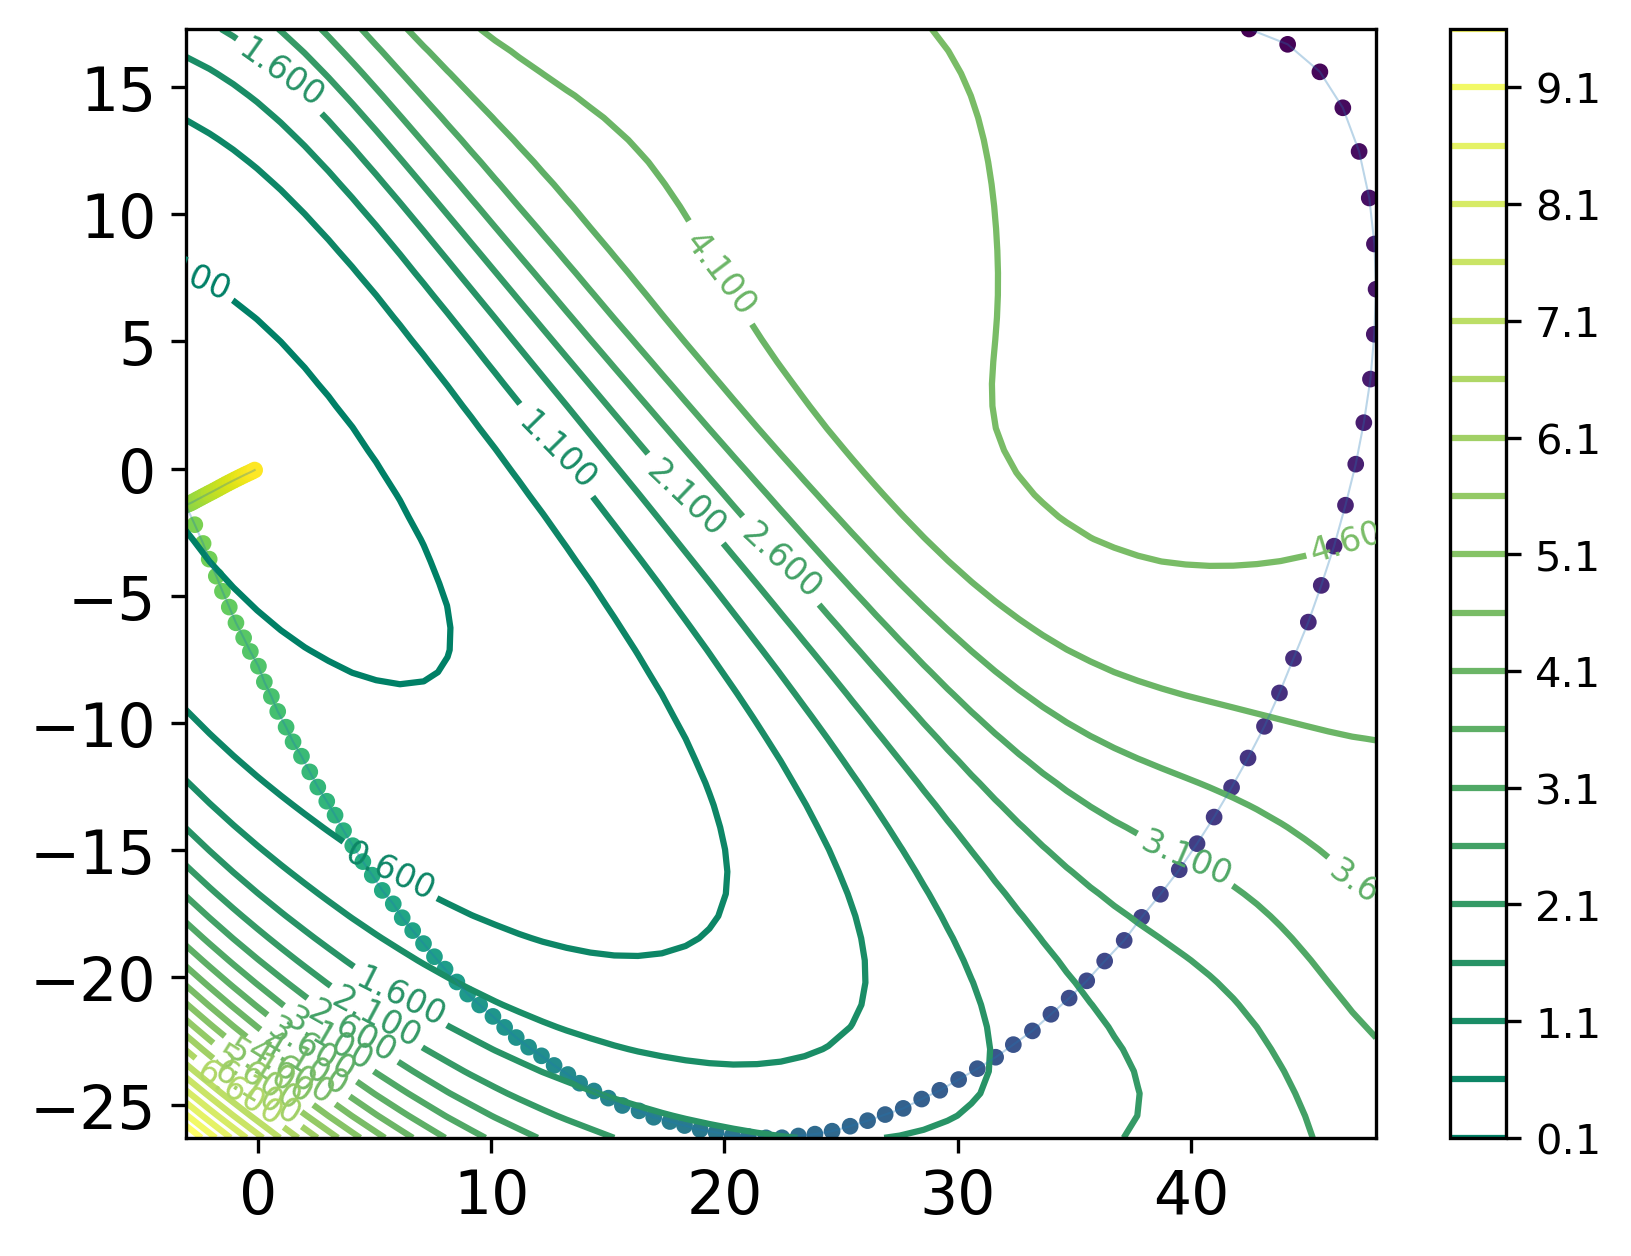
\includegraphics[width =  0.45\linewidth]{results/skip_conn/resnet20_with_final.png}} &
		\subfloat[Without Skip Connection]{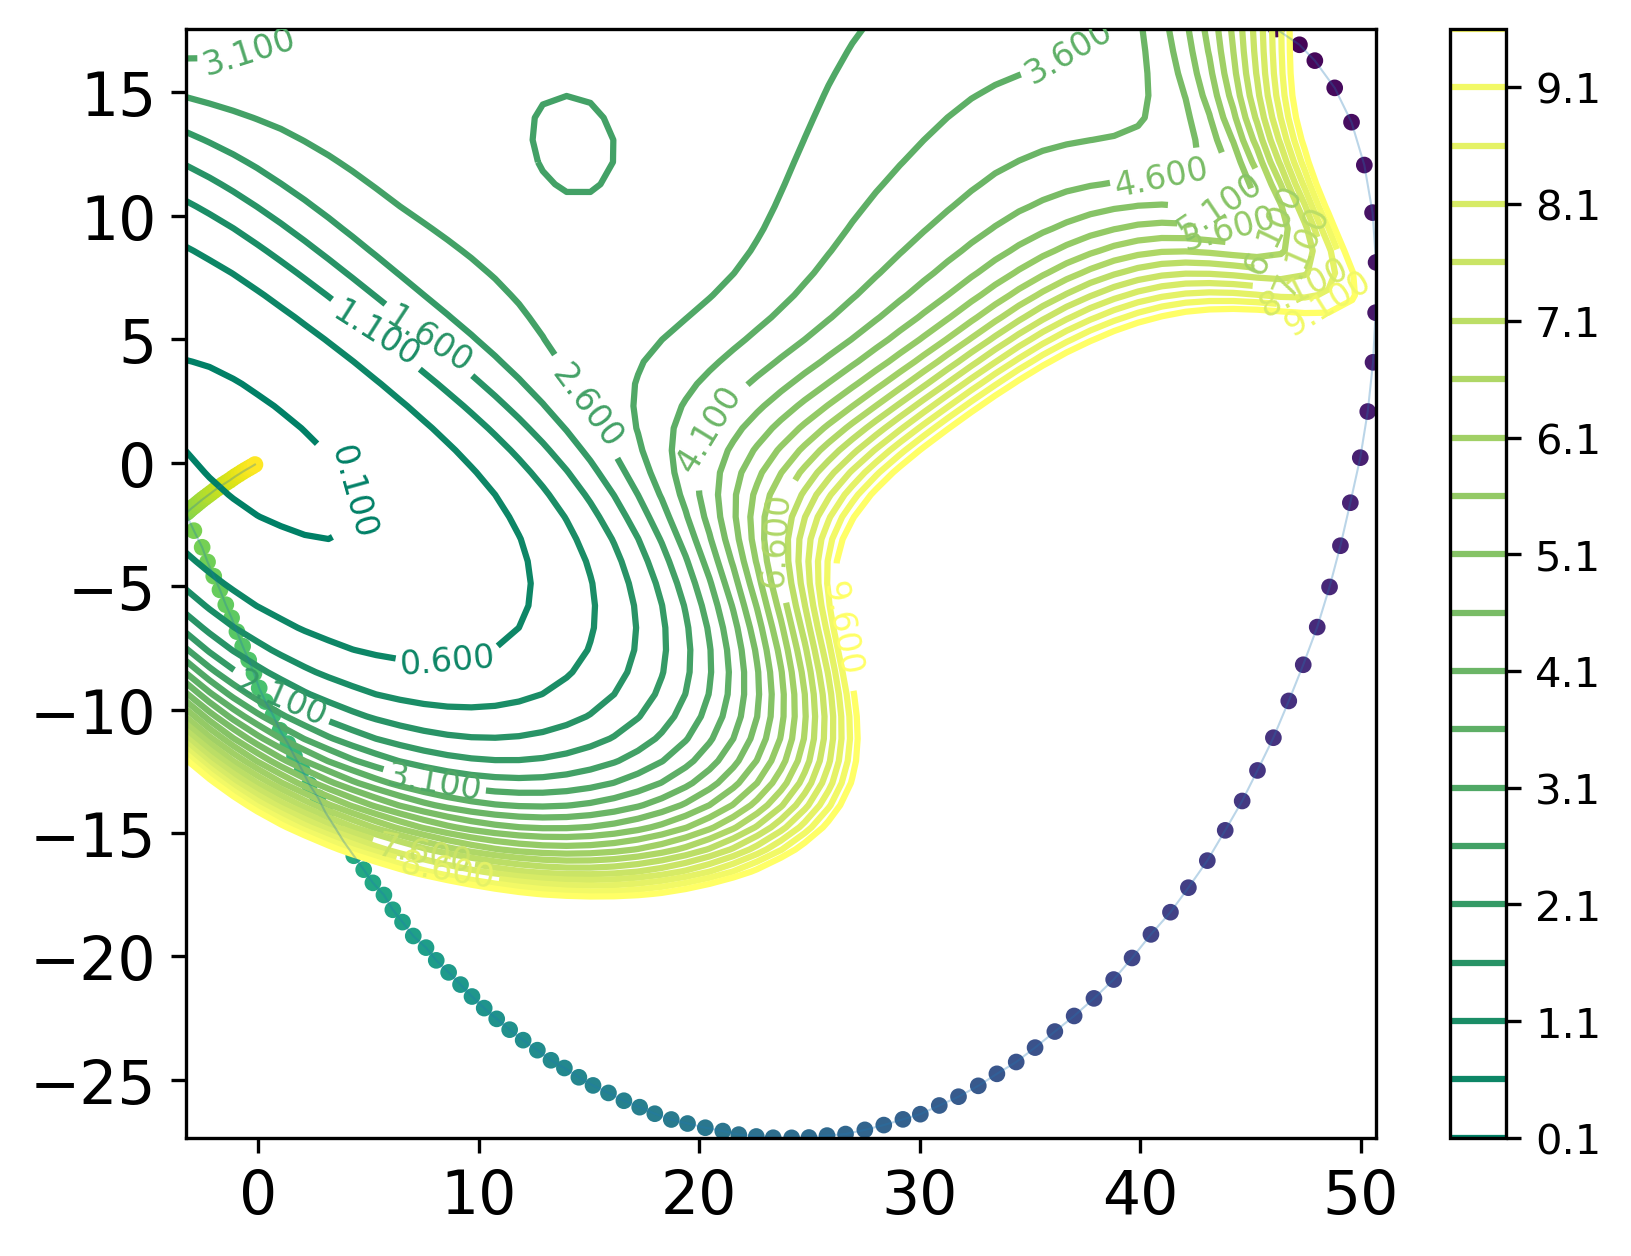
\includegraphics[width =  0.45\linewidth]{results/skip_conn/resnet20_without_final.png}} 
	\end{tabular}
	\caption{Loss landscape with/without Skip Connection (Trained)}
\end{figure}

%However, how does the landscape look at the initialization for these architectures?
Then, a natural question arise: would the skip connections ensure the smoother loss surface even prior to training? 
To this end, we picture the loss landscapes for the initialized weights with the same directions for projection in . 




%!TEX root=main.tex
\subsection{Data Augmentation}
\label{sec:data_augment}

In this group of experiments, we study the effects of two data augmentation methods: \textit{GaussianBlur} and \textit{ColorJitter}. 
\textit{GaussianBlur} will blur the input image with randomly chosen Gaussian kernels, while \textit{ColorJitter} changes the brightness, contrast, saturation and hue of an image.


\begin{figure}[htp]
	\label{fig:data_augment_final}
	\begin{tabular}{cc}
		\subfloat[With Data Augmentation]{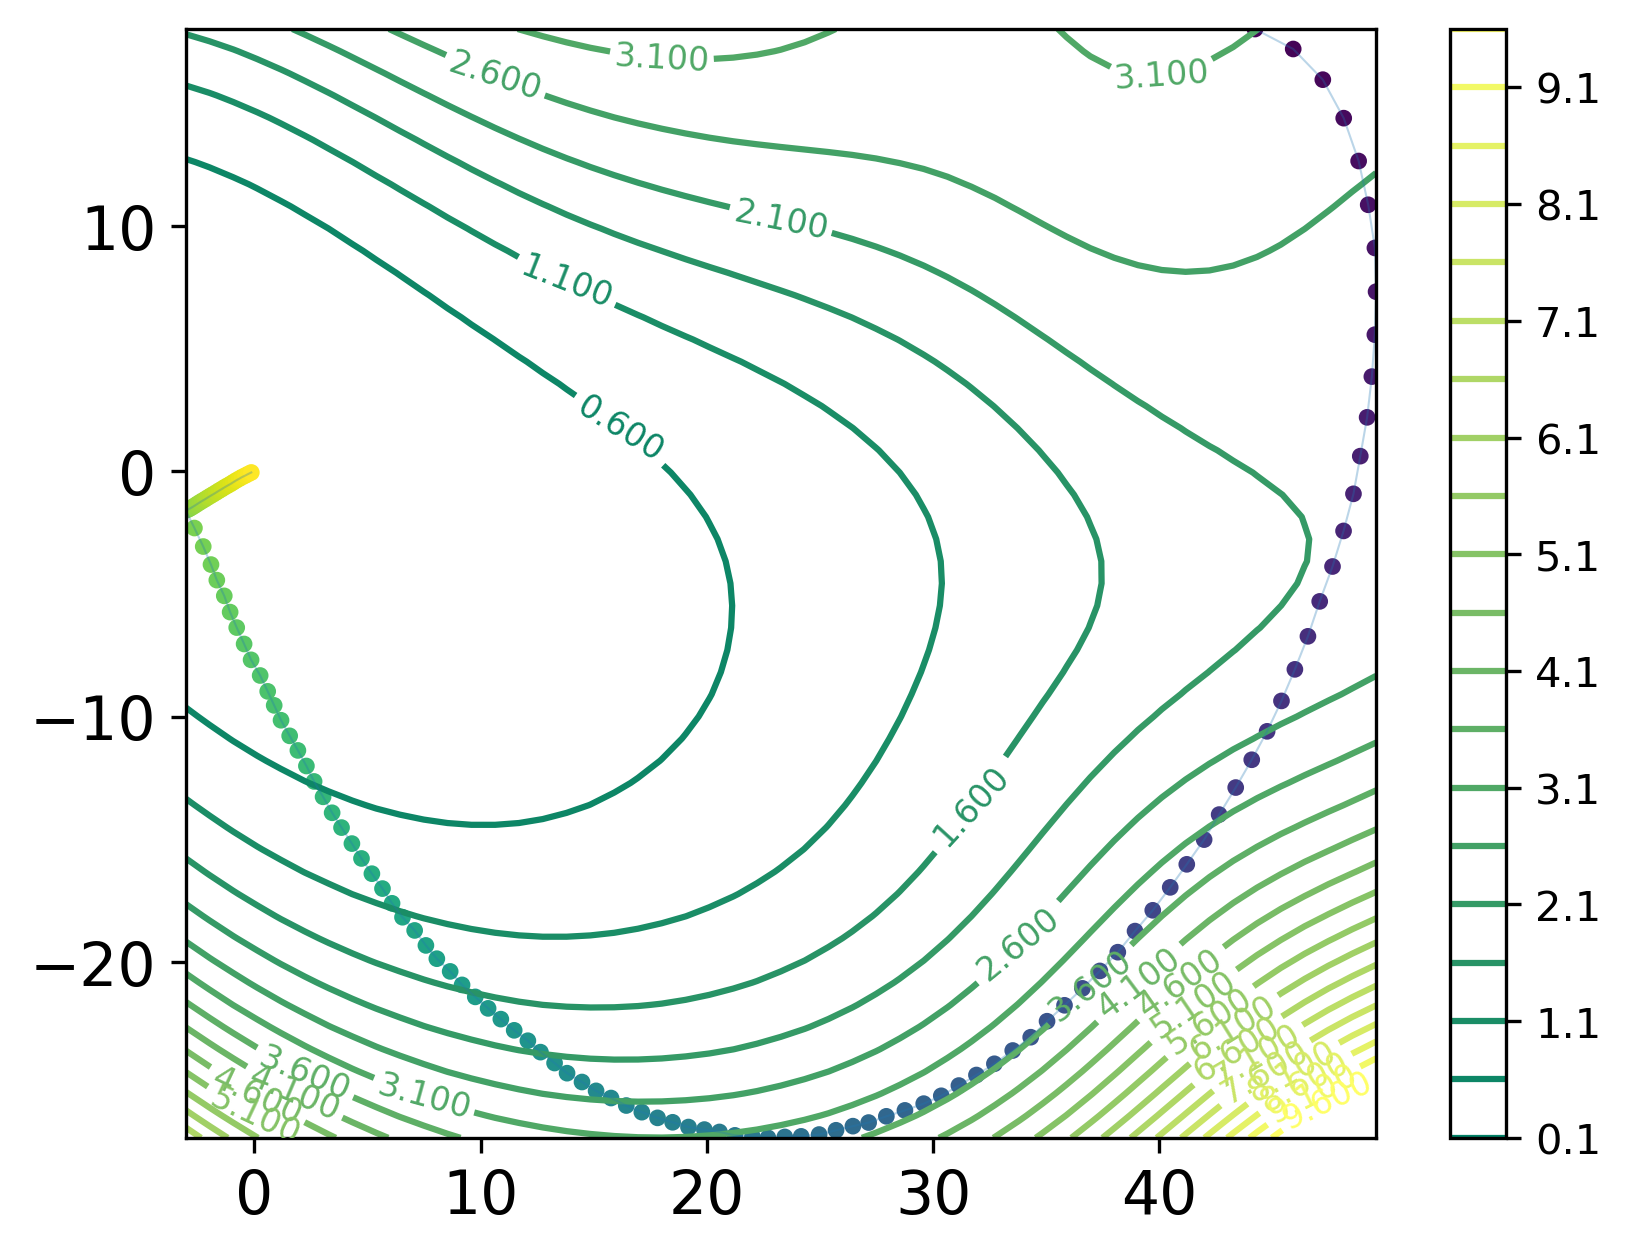
\includegraphics[width =  0.45\linewidth]{results/data_augment/resnet20_with_final.png}} &
		\subfloat[Without Data Augmentation]{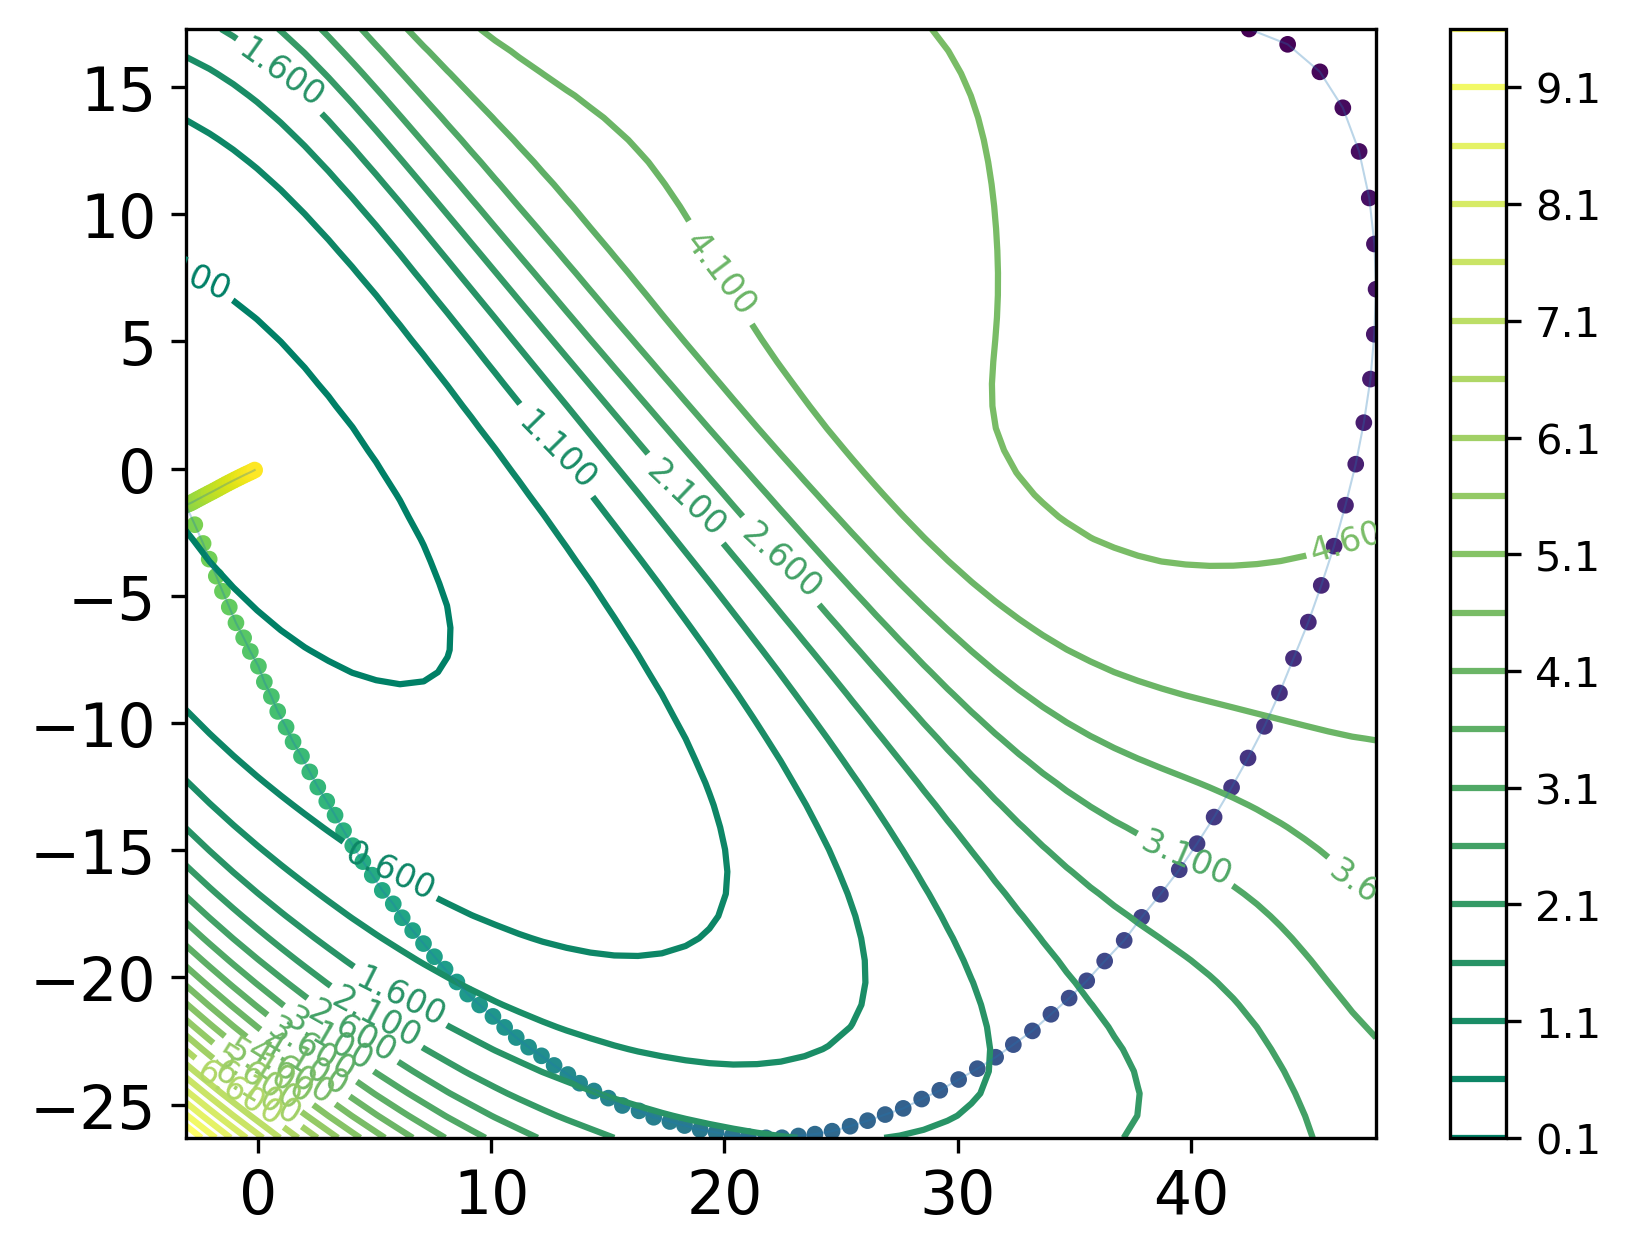
\includegraphics[width =  0.45\linewidth]{results/data_augment/resnet20_without_final.png}} 
	\end{tabular}
	\caption{Loss landscapes with/without Data Augmentation (Trained)}
\end{figure}

As expected, the extra data augmentation greatly improves the smoothness of loss surface, as the code of 

%!TEX root=main.tex
\subsection{Other Ideas}
\label{sec:others}
Within the original implementation, we found an interesting flag ``skip\_bn\_bias'' which is used for skipping batch norm and bias while computing the directions for projection and the loss landscape. 
We note that \cite{li2018visualizing} use this flag in their work without explanation. 
Thus, we wonder what could the loss landscape be like without this flag. 
Moreover, via this experiment, we shall see how the batch normalization layers keep the ``scale invariance'' property. 


%\begin{ack}
%\end{ack}

\bibliography{ref}
\bibliographystyle{plainnat}

%%%%%%%%%%%%%%%%%%%%%%%%%%%%%%%%%%%%%%%%%%%%%%%%%%%%%%%%%%%%


%%%%%%%%%%%%%%%%%%%%%%%%%%%%%%%%%%%%%%%%%%%%%%%%%%%%%%%%%%%%


\end{document}